\section{Introduktion}\label{sec:intro}
Denne aktivitet omhandler fremgangsmåden til opstilling og måling af overføringsfunktionen for en Buck-konverters udgangsfilter. De målte resultater sammenlignes med de beregnede amplitude- og fase-plots. Der inkluderes også brug af MATLAB, med et program som læser data fra en fil, og derved kan generere et bodeplot. \\
\\
Målet med denne aktivitet er, at få forståelse for overføringsfunktionen af en Buck-konverter. 
Aktiviteten er også med til at give et indblik i de forskellige MATLAB kommandoer, samt den generelle brug. 
Aktivitet skal ligeledes danne grundlag for aktivitet 2. 

\section{Teori}\label{sec:teori}
En overføringsfunktion er beskrevet ved forholdet mellem udgang og indgang. Her angivet i s-domænet
\begin{align}
	H(s) = \frac{V_{out}(s)}{V_{in}(s)}
\end{align}
\\
For at danne et udtryk for en overføringsfunktion ved en bestemt model, bruges almindelig kredsløbsanalyse. Kredsløbsanalysen indebærer at danne ækvivalent for serielle og parallelle forbindelser.

\begin{figure}[h!]
	\centering
	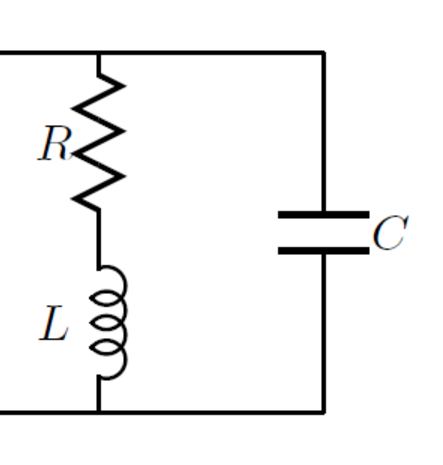
\includegraphics[width=.2\textwidth]{rlc.png}
	\caption{RLC-kredsløb}
	\label{fig:rlc}
\end{figure}

Betragt figur \ref{fig:rlc}. Her ses et \textbf{RLC}-kredsløb, som vil have ækvivalent $(R+L||C)$, der også kan udtrykkes som $\frac{C(R+L)}{C+R+L}$.
For at kunne opstille overføringsfunktionen for et sådant system, anvendes de komplekse impedanser 
\begin{align}
	Z_R &= R\\
	Z_C &= \frac{1}{sC}\\
	Z_L &= sL
\end{align} 
hvor $s = j\omega$ for det komplekse plan.
Således kan overføringsfunktionen for kredsløbet i figur \ref{fig:rlc} opstilles som
\begin{align}
	H(s) = \frac{V_{C}(s)}{V_{RL}(s)} = \frac{\dfrac{1}{sC}\left(R+ sL\right)}{\dfrac{1}{sC} + sL + R}
\end{align}
og den samme fremgangsmåde benyttes til opstilling af overføringsfunktionen for udgangsfilteret anvendt senere. 
\\\\
I en kondensator findes der en modstand kaldet ESR modstand som er en indre modstand der sidder i serie med kondensatoren. Tages denne ESR modstand med i den teoretiske model af kondensatoren, fremstår modellen tættere på en real kondensator og som det ses i de efterfølgende afsnit , har indflydelse på hvor nøjagtigt en model der kan opstilles for udgangsfilteret. 
